\documentclass[10pt]{article}
\pagestyle{plain}
\usepackage{fullpage,graphicx,float}
\usepackage[shortlabels]{enumitem}
\usepackage[labelfont=bf,textfont=it]{caption}
\usepackage[hyphens]{url}

\graphicspath{{fig/}}

\title{CSC 726: OpenMP Assignment}
\author{Irina Viviano and Ziqin Chen}
\date{}

\begin{document}
\maketitle

\begin{enumerate}

\item We ran \texttt{knapsack\_sequential.cpp} using different values of \texttt{capacity}
 and \texttt{numitems} to find out when the memory inefficient solution, memory efficient value, and memory efficient solution would have a running time of around 10 seconds. Table \ref{tab:10secs} below summarizes our findings.
 
 \begin{table}[h!]
 \begin{center}
 \begin{tabular}{|c|c|c|c|}
 \hline
 Algorithm & \texttt{capacity} & \texttt{numitems} & Time (seconds) \\
 \hline
 Memory inefficient solution & 100000 & 1800 & 10.5819 \\
 Memory efficient value & 1000000 & 400 & 10.3104 \\
 Memory efficient solution & 100000 & 1800 & 9.90371 \\
 \hline
 \end{tabular}
\caption{Capacity and number of items combinations in order to achieve a running time of around 10 seconds for each of the three algorithms.\label{tab:10secs}}
 \end{center}
 \end{table}

\item We created another file called \texttt{knapsack\_cache.cpp} which takes advantage of cache locality optimizations that improve the performance of the algorithms over the given sequential code.

We first noticed that the table is stored in a one-dimensional array, but uses linear indexing in order to access elements in order to mimic a two-dimensional storage scheme of the data. This is done in column-major order via the formula $w+j*(W+1)$ where $w$ is the row index, $j$ is the column index, and $W$ is the total number of rows. However, the doubly-nested for-loops in the \texttt{build\_table} function loop over the 2D table in row-major order, which does not take advantage of the spatial cache locality of the column-major linear indexing function. Therefore, our first change was to switch these for-loops so as to access the array elements in column-major order. 

We also noticed that in the \texttt{findk} function, column-major linear indexing was being used. However, since this function is part of the computation for the memory efficient solution, only four columns are being kept track of at a time, so the cache line is of length 4 and it makes sense to access the elements in row-major order so as to read in a line of cache every time. Therefore, we created a new linear indexing function that uses the formula $j+w*(N)$, where $N$ is the total number of columns. It is important to note that we are keeping track of two separate sets of two columns, and so when we call the linear indexing function, we pass in 2 as the value of $N$. 

The cache-optimized version of the algorithms indeed improves the performance, as summarized in Table \ref{tab:cache} below. Note that the memory inefficient cache optimization gives the most improvement, which corresponds to switching the order of the doubly-nested for-loops in the \texttt{build\_table} function.

 \begin{table}[h!]
 \begin{center}
 \begin{tabular}{|c|c|c|c|c|}
 \hline
 Algorithm & \texttt{capacity} & \texttt{numitems} & Time (seconds) & Speed-Up\\
 \hline
 Sequential Memory inefficient solution & 100000 & 1500 & 8.12009 & N/A \\ 
 Cache Memory inefficient solution & 100000 & 1500 & 4.20868 & 1.92936\\
 Sequential Memory efficient value & 100000 & 1500 & 3.52032 & N/A \\
 Cache Memory efficient value & 100000 & 1500 & 3.51614 & 1.00118  \\
 Sequential Memory efficient solution & 100000 & 1500 & 8.29262 & N/A \\
 Cache Memory efficient solution & 100000 & 1500 & 8.018 & 1.03425 \\
 \hline
 Sequential Memory inefficient solution & 100000 & 3000 & 19.371 & N/A \\ 
 Cache Memory inefficient solution & 100000 & 3000 & 8.4241 & 2.29947\\
 Sequential Memory efficient value & 100000 & 3000 & 6.91847 & N/A \\
 Cache Memory efficient value & 100000 & 3000 & 6.91169 & 1.00098  \\
 Sequential Memory efficient solution & 100000 & 3000 & 16.3221 & N/A \\
 Cache Memory efficient solution & 100000 & 3000 & 15.729 & 1.0377 \\
 \hline
 Sequential Memory inefficient solution & 1000000 & 300 & 11.4886 & N/A \\ 
 Cache Memory inefficient solution & 1000000 & 300 & 9.22011 & 1.24664\\
 Sequential Memory efficient value & 1000000 & 300 & 7.72272 & N/A \\
 Cache Memory efficient value & 1000000 & 300 & 7.72085 & 1.00024  \\
 Sequential Memory efficient solution & 1000000 & 300 & 18.5411 & N/A \\
 Cache Memory efficient solution & 1000000 & 300 & 18.0262 & 1.0288 \\
 \hline
  Sequential Memory inefficient solution & 2000000 & 30 & 1.78029 & N/A \\ 
 Cache Memory inefficient solution & 2000000 & 30 & 1.77115 & 1.0049619\\
 Sequential Memory efficient value & 2000000 & 30 & 1.53784 & N/A \\
 Cache Memory efficient value & 2000000 & 30 & 1.52932 & 1.00565  \\
 Sequential Memory efficient solution & 2000000 & 30 & 3.56975 & N/A \\
 Cache Memory efficient solution & 2000000 & 30 & 3.4692 & 1.029 \\
 \hline
 \end{tabular}
 \caption{The time and speed up for different capacity and number of items combinations for the original sequential algorithms and the cache optimized algorithms.\label{tab:cache}}
 \end{center}
 \end{table}


\item We created another file called \texttt{knapsack\_parallel.cpp} in order to parallelize the three knapsack algorithms. 

Note that in order to parallelize the component of the algorithm that computes the dynamic programming table, the operations must be independent and the data on which a particular entry depends needs to have already been computed and be available to all the processors. This can be accomplished by considering each column of the dynamic table sequentially, but filling in the entries of that column (i.e. the rows) in parallel. In this way, we can ensure that the values for which a particular entry depends (i.e. those in a previous column) have already been computed. Note also that the computation within the rows of one column are independent, since only values in the previous column need to be accessed. 

To accomplish this in the code, we first ensure that each set of doubly-nested for-loops that access the dynamic programming table loops over the items first (i.e. the columns) and the capacities second (i.e. the rows). Note we needed to switch the order of the loops in the \texttt{build\_table} function. Then, we simply placed a \texttt{\#pragma omp parallel for num\_threads(p)} in front of the second for-loop for each set of doubly-nested for-loops, where $p$ is the number of threads as specified by the user's command line input. 

We ran the parallel version of the knapsack algorithms for various combinations of capacity and number of items for different numbers of threads. The full raw data can be accessed in the file \texttt{output.txt}. We present in Figure \ref{fig:speedup} the speed-up of the three algorithm types for a capacity of 1,000,000 and 300 items with a varying number of threads. Table \ref{tab:speedup} summarizes the raw data. Observe that we gain significant increases in performance for the memory efficient algorithms, whereas the memory inefficient algorithm grows more slowly.

 \begin{figure}[!ht]
\centering
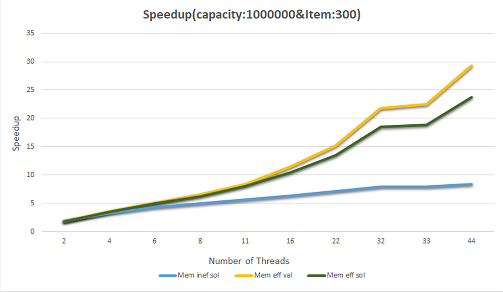
\includegraphics[width=1.01\textwidth]{speedup.pdf}
\caption{Speed-up for a capacity of 1000000 and 300 items for the parallel algorithms with a varying number of threads. \label{fig:speedup}}
\end{figure}

 \begin{table}[h!]
 \begin{center}
 \resizebox{\textwidth}{!}{\begin{tabular}{|c||c|c||c|c||c|c|}
 \hline
Number of Threads & \texttt{mem inef sol} Time (sec) & Speed-Up & \texttt{mem eff val} Time (sec) & Speed-Up & \texttt{mem eff sol} Time (sec) & Speed-Up\\
 \hline
1 & 11.4886 & N/A & 7.72272 & N/A & 18.5411 & N/A \\
2 & 6.12013 & 1.877182347 & 4.22523 & 1.827763222 & 10.4751 & 1.770016515 \\
4 & 3.57788 & 3.211007636 & 2.13773 & 3.612579699 & 5.30685 & 3.493805176 \\
6 & 2.68192 & 4.28372211 & 1.51009 & 5.114079293 & 3.77514 & 4.911367525 \\
8 & 2.33688 & 4.91621307 & 1.1769 & 6.5619169 & 2.96395 & 6.255537374 \\
11 & 2.01815 & 5.692639298 & 0.918686 & 8.406267212 & 2.318 & 7.998748921 \\
16 & 1.79884 & 6.38667141 & 0.676357 & 11.41811203 & 1.77596 & 10.44004369 \\
22 & 1.60412 & 7.161933022 & 0.508205 & 15.19607245 & 1.36992	 & 13.53443997 \\
32 & 1.45265 & 7.908718549 & 0.353914 & 21.82089434 & 1.00318 & 18.4823262 \\
33 & 1.45289 & 7.907412123 & 0.344011 & 22.44904959 & 0.980722 & 18.90556141 \\
44 & 1.36842 & 8.395521843 & 0.263671 & 29.28922786 & 0.781908 & 23.71263627 \\
 \hline
 \end{tabular}}
 \caption{The time and speed up for a capacity of 1000000 and 300 items for the parallel algorithms with a varying number of threads.\label{tab:speedup}}
 \end{center}
 \end{table}

\end{enumerate}


\end{document}